\chapter{Criptosistemas clásicos}

Problema a solucionar:

\begin{figure}[h]
	\begin{center}
		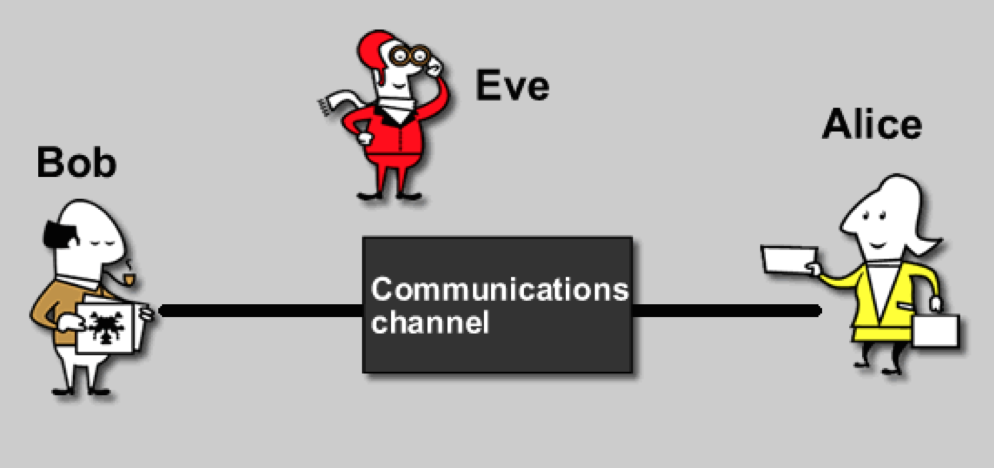
\includegraphics[width=0.5\textwidth]{img/aliceBobEve.png}
	\end{center}
\end{figure}


El problema radica en enviar un mensaje por un canal al que E tiene accesso. Hay que resolver problemas tanto de confidencialidad como de identificación.

\textbf{Primeras soluciones}

	\section{Esteganografía}

		Intentar ocultar la existencia del mensaje. Es un método con origen muy antigüo (~486-425 a.C)

	\section{Criptografía}

		Intentar que el mensaje no se pueda leer aunque se intercepte. También tiene unorigen muy antigüo (~500 a.C)

		La mayoría de estos métodos se basaban en transposición.

		\begin{defn}[Transposición]
			Cambio en el orden de las letras de un mensaje
		\end{defn}

		\subsection{El criptosistema de Cesar}

			Se utiliza la sustitución como método de encriptación, normalmente cambiando cada letra por su correspondiente al desplazarse \texttt{d} espacios atrás en el abecedario. Por ejemplo:

			\begin{tabular}[h]{c|c}
			sin cifrar & cifrado \\ \hline
			A & D\\
			B & E\\
			C & F\\
			... & ...
			\end{tabular}

		\subsection{Formalización}

		Hay dos colecciones de mensajes:

		\begin{enumerate}
			\item M = Mensajes en claro
			\item C = Mensajes cifrados
		\end{enumerate}

		Un alfabeto, o dos, si el alfabeto de M y el de C son distintos:

		\begin{itemize}
			\item $A = \{A,B...Z\}$
			\item $A = \{0,1\}$
			\item $A = \{A,B...Z,\hdots,\text{?`},\text{?},1,2,3,\hdots,9,0\}$
			\item $A = $ Código ASCII 
		\end{itemize}



		Funciones para cifrar:

		$f: M \rightarrow C$ inyectiva

		La correspondiente función para descifrar sería:

		$f^{-1}: C \rightarrow M$


		A debe conocer $f$ y $B$ debe conocer $f^{-1}$. A envía un mensaje $m\in M$ a $B$ usando $f(m)=c$ y enviando $c$. $B$ puede obtener el mensaje calculando $f^{-1}(c) = m$.

		En este modelo, romper el sistema de cifrado equivale a que un tercero averigüe $f^{-1}$.


		\textbf{¿Podemos usar más de una función para cifrar?}

		En el sistema de Cesar se puede cambiar, por ejemplo, la longitud desplazmiento por el abecedario al realizar la encriptación, aunque no hay muchas posibilidades.


		\begin{defn}[Criptosistema]
			Colección de functiones para fifrar:

			$f_e : M_e \rightarrow C_e$

		\end{defn}


		\vspace{1.5cm}

		\begin{example}{Como romper la criptografía Cesar}
		
			Se puede romper "facilmente" la criptografía Cesar con análisis de frecuencias. Por ejemplo, en castellano la letra más frecuente es la E, con un 13,68\%, sabiendo la letra más frecuente de un mensaje cifrado se puede calcular la distancia entre esa y la E y muy probablemente hayamos hallado la clave de cifrado.

			La fiabilidad de este método puede verse mermada por la genericidad del texto cifrado. Si es corto y si habla de un tema en particular es posible que las frecuencias varíen respecto a otros textos genéricos en Español.

			De hecho, por ejemplo, en el manual de UNIX la frecuencia de la letra e baja al 9\% dejando a la letra relegada al cuarto puesto, por detrás de la t, la n y la i.

		\end{example}


		Veamos la frecuencia general de distintos grupos de letras en ingles.

		\begin{tabular}[h]{r|c|c}
			\textbf{grupos} & \textbf{frec} & \textbf{rango} \\ \hline
			e & 12.7\% & 12.7 \\
			taoiushr & 56.9 & 6-9 \\
			cumwfgypb & 19.9 & 1.5 - 3 \\
			vkjxqz & 2.2 & < 1
		\end{tabular}

		\section{Criptosistema afín (sobre letras)}

			Alfabeto de N letras $\leftrightarrow \mathbb{Z}/N$

			Claves: $a,b \in \mathbb{Z}/N$

			\begin{align*}
				f_{a,b} :&  \mathbb{Z}/N\to \mathbb{Z}/N\\
				& x \rightarrow ax + b
			\end{align*}

			¿Para qué valores de a,b es $f_{a,b}$ inyectiva?

			Calculamos $f^{-1}_{a,b}$

			$$ax+b = y$$
			$$ax = y - b$$

			Si $a \in U(\mathbb{Z}/N)
			\implies 
			x = a^{-1} (y-b) \implies 
			x = a^{-1}y - a^{-1}b$
			

			$$f^{-1}_{a,b} = f_{a^{-1},-a^{-1}b}$$

			Así hemos demostrado que:

			\begin{enumerate}
				\item $a \in U(\mathbb{Z}/N) \Rightarrow f_{a,b}$ inyectiva
				\item En ese caso si $e = (a,b)$ es la clave para cifrar $\Rightarrow d = (a^{-1},-a^{-1}b)$ es la clave para descifrar.
			\end{enumerate}

			Usando la definición de inyectiva:

				$$ \exists \alpha \in q : a \alpha = 1 \Leftrightarrow a \alpha + b = 1 + b $$

			Así llegamos a la conclusión de que en realidad el par $(a,b)$ tiene ciertas restricciones:

			$$ E = \{ (a,b): a \in U(\mathbb{Z}/N), b \in \mathbb{Z}/N \} $$

			$$ \#E = \#U(\mathbb{Z}/N) * \#\mathbb{Z}/N $$


			\begin{prop}
				Sea $a \in \mathbb{Z}/N : a \in U(\mathbb{Z}/N) \Leftrightarrow (a,N) = 1$ (son primos entre si).

				\begin{proof}

					\textbf{$\Rightarrow$}

					$$\exists \alpha \in \mathbb{Z}/N : a \alpha \equiv 1 \mod n \Rightarrow \exists k : a\alpha + kN = 1$$

					$$\text{Si } (a,N) \neq 1 \Rightarrow \exists p \text{ primo } : p | a, N \Rightarrow p | ax + 1 (FALTA UN PELÍN)$$

					\textbf{$\Leftarrow$}

					$(a,n) = 1$. Esto se demuestra usando el algoritmo de euclides. 

				\end{proof}
			\end{prop}


			Volvemos entonces al número de claves ya que sabemos como calcularlo:

			$$ \#E = \#U(\mathbb{Z}/N) * \#\mathbb{Z}/N = \phi(N)*N $$


			\subsection{La función de euler}

				$\phi(p) = p-1$

				$\phi(p^n) = p^{n} - p^{n-1} = p^{n-1} p(p-1) = p^{n}(1- \frac{1}{p})$

				Como es una función multiplicativa:

				$\phi(N) =N \Pi \phi(P_i^{n_i}) = \Pi P_i^{n_i} n_i \Pi (1- \frac{1}{p_i}) = N \Pi(1 - \frac{1}{p_i})$









\begin{figure}[h]
	\begin{center}
		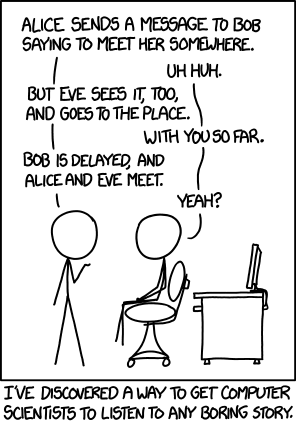
\includegraphics[width=0.5\textwidth]{img/protocol.png}
	\end{center}
\end{figure}



